\chapter{Introduction}
\section{Motivation}\label{sec:motivation}
Whether it be water in a pipeline, or an aircraft soaring through the skies, every fluid passing by a solid and every solid passing through a fluid will experience drag. The ever pressing need to reduce our impact on the environment requires us to reduce our energy used to combat unwanted drag, which also has the added benefit of reducing costs via increased efficiency. This is especially true in the transportation sector, which accounted for 24\% of total global emissions in 2019 according to the IEA, although growth has been limited to only 0.5\% per year compared to an average increase of 1.9\% annually since 2000 owing to efficiency improvements \cite{iea2021}.

The search for these efficiency improvements includes research towards \gls*{dr} via flow control -- that is manipulating the flow characteristics in such a way that somehow produces less overall drag. In fact, Ludwig Prandtl, who revolutionised the study of fluid mechanics with the introduction of the \gls*{tbl}, pioneered modern flow control as early as 1904, where he demonstrated that suction at the surface of a cylinder delays \gls*{bl} separation and therefore decreases drag \cite{gad-el-hak2001,prandtl1904}. Indeed, \gls*{dr} is a major focus of research in commercial aviation. In the context of aviation, a 1\% reduction in drag corresponds to a 0.75\% reduction in fuel and as a result \ensuremath{\mathrm{CO_2}} emissions \cite{leschziner2011}. In fact, \textcite{leschziner2011} states that based on estimates on travel demand in 2030, a 1\% reduction will constitute a 9 million tonnes reduction in \ensuremath{\mathrm{CO_2}} emissions.

In transport applications, and in particular aviation, the flows are at high Reynolds numbers \gls*{re}, this means the regimes we are dealing with are often turbulent. Moreover, especially in aviation (with the exception of cases where supersonic effects dominate), viscous drag generated in the near-wall \gls*{bl} region constitutes a major component of total drag \cite{abbas2017}. These two factors combined mean that ``flow control methodology targeting the \gls*{tbl} is the most obvious option to achieve a significant skin-friction-drag reduction and ultimately to reduce emissions" \cite{abbas2017}.

Flow control is separated into two distinct groups, active and passive control. Active flow control requires an input in energy to affect the flow via the use of actuators, whereas passive flow control does not. Examples of active control include opposition control \cite{choi1994,luhar2014}, spanwise-wall oscillation \cite{jung1992,choi1998,viotti2009}, and the aforementioned \gls*{bl} separation control \cite{prandtl1904}; the former is closed-loop and reacts to sensor inputs from the environment, whereas the latter two can be either open-loop with predetermined control patterns or reactive (feedback/feed-forward systems). The actuators used to perform active flow control can range from zero-net-mass-flux jets \cite{zhang2008}, to dielectric-barrier-discharge plasma actuators \cite{wang2013}, to fluid injection (blowing) and sucking \cite{chng2009}, to the ingenious moving surface using ``pneumatically actuated compliant structure based on the kagome lattice geometry'' \cite{bird2018}.
Whereas, examples of passive control include vortex generators \cite{chang1970}, discontinuities/notches/fences in the leading/rear edges of a wing \cite{chang1970}, compliant surfaces \cite{choi1997}, porous coatings \cite{klausmann2017}, superhydrophobic surfaces \cite{truesdell2006}, and a very well studied control technique known as riblets \cite{walsh1983,choi1993,garcia-mayoral2011}.

As aforementioned, active flow control allows for reactive responses which can increase the effectiveness of control techniques. Moreover, even open-loop flow control can achieve higher viscous drag reduction than passive control techniques without the need for sensors required for reactive flow control. However, this comes at a cost of the extra energy expended to modify the flow and the difficulty and innovation needed to design actuators. This can clearly be seen in the case of spanwise-wall oscillation where the wall moves as prescribed by a streamwise travelling wave, which, after accounting for the power spent to oscillate the fluid, has a net power saving of around 26\% despite a drag reduction of $>35\%$ for those conditions \cite{quadrio2009}. Moreover, in order to emulate a in-plane wall motion in real life, the aforementioned compliant structure from \cite{bird2018} had to be created and trialled in laboratory conditions, and then made at scale and maintained if it were to be used on real-world flows.

On the other hand, passive flow control in necessarily open-loop, and may have decreased performance in comparison to active flow control. However, it does not require actuators and the maintenance thereof. Riblets, for example, ``are small surface protrusions aligned with the direction of the flow, which confer an anisotropic roughness to a surface'' \cite{garcia-mayoral2011} and can be seen in Figure~\ref{fig:riblets}. Experiments show that under moderate adverse pressure gradient (i.e. where the pressure increases along the direction of the flow) a 13\% skin friction reduction is achievable, compared to 6\% reduction in a zero-pressure-gradient \gls*{bl} \cite{debisschop1996}. Although less efficient compared to active control, due to its relatively simple design, its \gls*{trl} is higher than most other flow control techniques. In fact it has been trialled in scale model aircraft tests in transonic Mach numbers \cite{coustols1990}, real aircraft tests, and even in commercial service for several years by Cathay Pacific on an Airbus A340 where 30\% of the wetted surface was covered with riblets \cite{bechert2006}. Based on a flight test on an Airbus A320, in transonic Mach number ranges, an A320 with 70\% of the wetted surface covered by riblets could have a drag reduction of about 2\% \cite{szodruch1991}. However, the optimal grove cross section was found to have an optimum at $\left(\gls*{garea}\right)^{1 /2}\approx11$, where the $+$ superscript denotes non-dimensionalisation by wall units (see~\ref{sec:ssl}) and spacing of approximately 15 wall units \cite{garcia-mayoral2011}. This is equivalent to approximately \SIrange{30}{70}{\micro\metre} in realistic aerofoil and aircraft flows \cite{garcia-mayoral2011}. Moreover, the sharper the riblets, the more efficient they are at reducing drag \cite{garcia-mayoral2011}. All of these factors make riblets quite hard to manufacture whilst requiring maintenance/replacements due to the erosion from air moving past.

\begin{figure}[htbp]
\centering
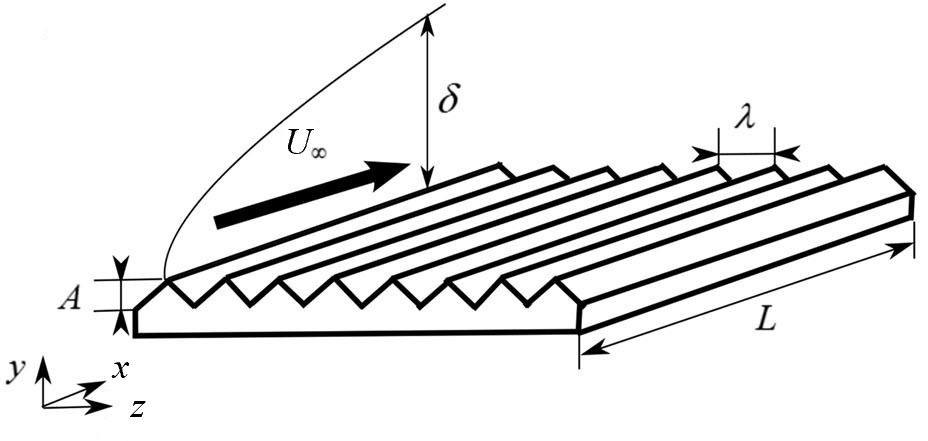
\includegraphics[width=0.5\linewidth]{introduction/fig/riblets.jpeg}
\caption[Schematic of triangular riblets]{A schematic of triangular riblets; the most commonly researched riblets. Figure modified from \cite{raayai-ardakani2019}.}
\label{fig:riblets}
\end{figure}

Therefore, researchers have begun to explore other ways to use passive flow control for turbulent \gls*{dr}. The oblique \gls*{ww} was first proposed by \textcite{chernyshenko2013} in 2013 to emulate the motions of in-plane spanwise wall oscillations in hopes that there will be a net energy decrease. We will devote the rest of this report discussing the merits of this curious passive flow control method.

%It is known that if in a turbulent flow the (wing) surface moves spanwise with a suitable velocity distribution, the friction drag is significantly reduced. Even though causing the wing surface to move requires energy input, the drag reduction is large enough to provide large energy savings. However, such motion is difficult to implement on an aircraft. In a paper (Chernyshenko, 2013, arxiv.org/abs/1304.4638) it was proposed to shape the rigid (not moving) surface in such a way that the resulting fluid motion will emulate the effect of the surface motion without the surface actually moving. For the case of the surface with sinusoidal waves at an angle to the mean flow direction, an optimisation of the angle and the height of the waves was performed. The later comparisons (Ghebali et al., 2017, aip.scitation.org/doi/10.1063/1.5003617) showed that the semi-empirical model of calculating the drag reduction used for optimisation was inaccurate. This might be due to this model not taking into account the energy dissipation due to the laminar viscosity and the shape of the mean velocity profile. This part of the dissipation is negligible at high Reynolds numbers, but it was significant at the Reynolds numbers studied. The project will consist in improving the semi-empirical model and repeating the shape optimisation using the improved model. It is recommended to see the first paper cited above to estimate the degree of mathematical proficiency needed for this project.

\section{Literature Review}
\subsection{The Spatial Stokes Layer (SSL)}\label{sec:ssl}
\subsubsection{Description}
The Stokes layer is one of the few known exact solutions to the Navier-Stokes equation describing the motion of a viscous fluid as a function of the wall normal coordinate $y$, whereby the infinitely long wall is located at the bottom at $y=0$ and oscillating harmonically in its own plane \cite{schlichting2016}. It turns out that the resulting oscillation in the fluid is only of significant magnitude very close to the wall in a so-called ``Stokes layer'' and is significantly damped outside of the said-layer.

\citeauthor*{jung1992} \cite{jung1992} were the first to suggest using a wall oscillating in the spanwise direction to reduce skin friction in 1992, exploiting the above phenomenon to obtain a maximum drag reduction of 40\% at a non-dimensional period of $T^+=100$ using \gls*{dns}, a \gls*{cfd} method \cite{karniadakis2003}. The $+$ superscript denotes non-dimensionalisation by wall units, which is based upon the wall friction velocity $\gls*{ut}=\sqrt{\frac{\gls*{tw}}{\gls*{ro}}}$, along with the kinematic viscosity $\gls*{nu}=\frac{\gls*{mu}}{\gls*{ro}},$ where \gls*{tw} is the wall shear stress of the fluid flow, \gls*{ro} is the density of the fluid, and \gls*{mu} is the dynamic viscosity of the fluid flow. The spanwise velocity of the wall is given by
\begin{equation}
	\gls*{spanwv} = \gls*{awall}\sin{\left( \frac{2\pi}{\gls*{per}}\gls*{tim} \right)}
,\end{equation}
where \gls*{awall} and \gls*{per} denotes the oscillation amplitude and period, and \gls*{tim} denotes time.
Moreover, when only one of the channel walls were oscillating, ``the reduction in turbulence activity was observed only near the oscillating wall, while the flow at the other wall remained fully turbulent'' \cite{jung1992}. When phase averaged this coincides with the Stokes layer with temporal forcing \cite{viotti2009}, we will therefore name it \gls*{tsl}. \textcite{dhanak1999} observed that the duration of sweep events were reduced by 47\% and their strength reduced by 23\%, suggesting that the skin-friction reduction is a result of the ``attenuation in the formation of streamwise streaks \cite{karniadakis2003}.
%\textcite{karniadakis2003} provides an excellent review of research in in-plane wall motion up to 2003. 

As this is a form of active flow control, despite significant drag reductions, significant energy must also be expended to overcome the extra shear stress to create the spanwise motion of the fluid \cite{viotti2009}. \textcite{baron1996} was the first to consider the net energy savings from spanwise wall oscillation, and it is now accepted that the net energy savings is 10\% \cite{viotti2009, karniadakis2003}. However, this technique requires moving parts and therefore requires actuators, which is hard to implement in practical applications especially in transport applications.

\textcite{viotti2009} sought to extend the \gls*{tsl} from a time-dependent forcing to a stationary, spatial forcing, which potentially allows an extension into passive solutions which can emulate the oscillation varying over space instead of time (such as the \gls*{ww}). %(------------------------------------------------------------------------------------------------------------------------------------------ kim and hussain--------------------------------???)
Letting $x$ be the streamwise coordinate, $y$ the wall-normal coordinate, and $z$ the spanwise coordinate, the spatial forcing law can be seen in Figure~\ref{fig:ssl}, and is given by
\begin{equation}
	\gls*{spanwv} = \gls*{awall}\sin{\left( \frac{2\pi}{\gls*{lm}_x} x \right)} 
,\end{equation}
where \gls*{awall} and $\gls*{lm}_x$ denotes the forcing amplitude and the forcing wavelength in the $x$ direction respectively. We will call this flow the \gls*{ssl}.

\begin{figure}[htbp]
	\centering
	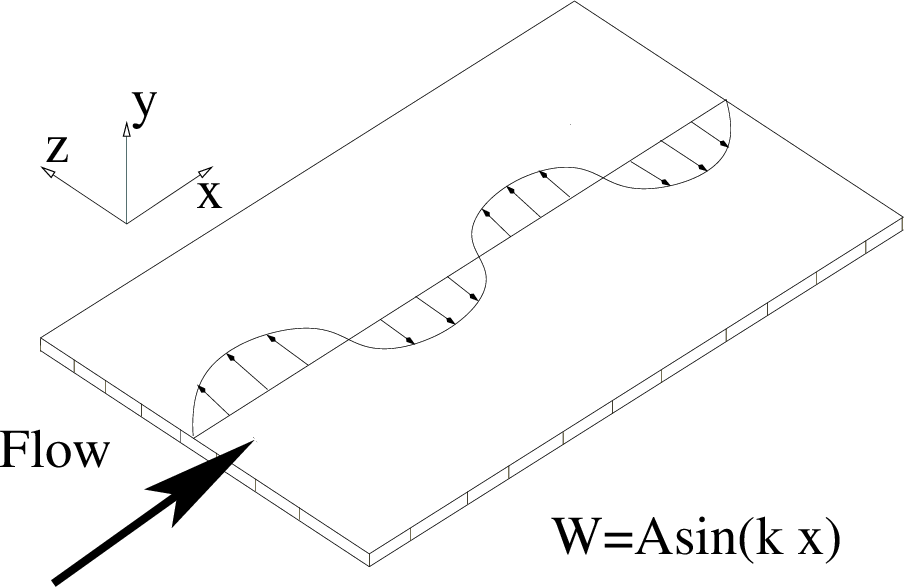
\includegraphics[width=0.5\linewidth]{introduction/fig/ssl.png}
	\caption[Schematic of spanwise wall forcing]{Schematic of spanwise wall forcing from \cite{viotti2009}.}
	\label{fig:ssl}
\end{figure}

\subsubsection{Solving for Velocity}
We will now analyse \gls*{ssl} flow analytically following \textcite{chernyshenko2013}, who ultimately derives their analysis from \textcite{viotti2009}. We begin by solving for the velocity profile of \gls*{ssl} flow by first defining the triple decomposition of velocity as follows
\begin{equation}
	\mathbf{U} = \overline{\mathbf{U} }+\tilde{\mathbf{u} }+\mathbf{u'}  
,\end{equation}
where $\overline{\mathbf{U} }$ is the velocity averaged over time, and space in the $x$ and  $z$ direction, $\tilde{\mathbf{u} }$ is the phase averaged velocity, and $\mathbf{u'} $ is the remaining stochastic turbulent part of the velocity. Unlike the traditional Reynolds decomposition, we have an extra phase dependent term, which is useful for periodic flows such as \gls*{ssl} flow. We can adapt the definition given in \cite{baj2015} to our case and define for some phase angle $\gls*{phase}_0=\gls*{phase}\left(x_0+m \gls*{lm}_x,z_0+n \gls*{lm}_z\right)$,
\begin{equation}
	\tilde{\mathbf{u} }\left(y,\gls*{phase}_0\right)\equiv\lim_{M\to\infty}\lim_{N\to\infty}\frac{1}{M}\frac{1}{N} \sum_{m=1}^{M} \sum_{n=1}^{N} \mathbf{U}\left(x_0+n \gls*{lm}_x,y,z_0 +m \gls*{lm}_z\right)-\overline{\mathbf{U} }(y)  
.\end{equation}
By including this average, we recognise that there will be periodicity in the $x$ component of the flow velocity; we also include periodicity in the $z$ component of the flow velocity since it will be useful for the \gls*{ww} flow, and doesn't affect the definition for the \gls*{ssl} flow, whose phase average has no $z$ dependence and therefore $\tilde{w}=0$.

Similarly, we can decompose the pressure field as we did velocity into its triple decomposition with $\gls*{press}=\gls*{mpress}+\gls*{ppress}+\gls*{fpress}$, where \gls*{mpress} is the mean pressure (averaged in time, $x-z$ space, and phase), \gls*{ppress} is the periodically fluctuating phase averaged pressure, and \gls*{fpress} is the randomly fluctuating pressure.

With that definition, we can now solve for the phase averaged velocity of the \gls*{ssl} flow. By linearising the \gls*{bl} equations in the wall units of the flow around a linear profile, we ignore the stochastic fluctuations $\mathbf{u'} $ and $p'$, and let $\overline{\mathbf{U} }^{+} = (y^{+},0,0)$. Moreover, \gls*{ssl} is time invariant. Thus, by analysing the order of various values as in \cite{schlichting2016}, and taking $\gls*{re}\to \infty$, we get
\begin{align}
	y^{+} \pdv{\tilde{u}^{+}}{x^{+}} + \tilde{v}^{+} &= -\pdv{p^{+}}{x^{+}} + \pdv[2]{\tilde{u}^{+}}{\left(y^{+}\right)} \label{eq:blx}\\
	0 &= -\pdv{p^{+}}{y^{+}}  \label{eq:bly}\\
	y^{+} \pdv{\tilde{w}^{+}}{x^{+}} &= -\pdv{p^{+}}{z^{+}} + \pdv[2]{\tilde{w}^{+}}{\left( y^{+} \right) } \label{eq:blz}\\
	0 &= \pdv{\tilde{u}^{+}}{x^{+}} +\pdv{\tilde{v}^{+}}{y^{+}} +\pdv{\tilde{w}^{+}}{z^{+}} \label{eq:blc}
.\end{align}
These are the general \gls*{bl} equations (also known as \textit{Prandtl \gls*{bl} equations}) when linearised around a linear mean profile (i.e. where we let $\overline{U}^{+}=\left(y^{+},0,0\right)$).

%(-----------------------------------------------------------Comparison between laminar and turbulent mean fields: Fig 3 Viotti------------------------------------------------)

At the wall ($y\ps=0$), we have $\tilde{u}\ssl\ps=\tilde{v}\ssl\ps=0$, and $\tilde{w}\ssl\ps=\gls*{wht}\ps e^{i \gls*{wnum}_x\ps x\ps}$, where $\gls*{wht}\ps\ssl=A\ps$ is the wall oscillation amplitude, $\gls*{wnum}_x\ps = \frac{2\pi}{\lambda_x\ps}$ is the non-dimensional wavenumber, $i$ is the imaginary unit, the subscript $\gls*{sl}$ denotes that the variable is related to \gls*{ssl} flow, and the superscript $+\gls*{sl}$ denotes non-dimensionalisation by the friction velocity specific to the \gls*{ssl} flow $u_{\tau,\gls*{sl}}=\sqrt{\frac{\tau_{w,\gls*{sl}}}{\gls*{ro}}} $, where $\tau_{w,\gls*{sl}}$ is the time, space, and phase averaged wall shear stress of the  \gls*{ssl} flow. Although strictly speaking this $\tilde{w}\ssl\ps$ at the wall is only the real part of the exponential function (as well as any other phase averaged terms that we prescribe the exponential function for the rest of this report), however analysis is much more easily done using the exponential function and only taking the real part thereof at the very end. Moreover, since the wall is flat, we expect the pressure gradient in all directions to be zero. We also only expect the spanwise periodic fluctuations to be non-zero, therefore $\tilde{u}\ssl=\tilde{v}\ssl=0  $. This means that to solve for $\tilde{w}\ps$ we only need Equation~\eqref{eq:blz}.

Finally, we expect the spanwise velocity to vary not only in $x$ (due to the  $x$ dependence of the prescribed spanwise wall forcing), but also in  $y$ as the Stokes layer decreases in strength away from the wall. Therefore, we get
\begin{equation}
	\tilde{w}\ps\left(x\ps,\check{y}\ps\right)=\gls*{wht}\ps\ssl\check{w}\ssl\ps e^{ik\ps_x x\ps}\label{eq:wtlddef}
,\end{equation}
where we define $y^{+}=\left(k^{+}_x\right)^{-1 /3}\gls*{yck}$ in order to simplify or equations later, and $\check{w}\ssl \ps=\check{w}\ssl \ps(\check{y}\ps)$ as the only part of $\tilde{w}\ps$ dependent on $\check{y}\ps$.\glsadd{wck}
Therefore Equation~\eqref{eq:blz} becomes
\begin{align}
	\left( k_x\ps \right) ^{-1 /3} \check{y}\ps \pdv{x\ps}(\hat{W}\ps \check{w}\ps\ssl e^{ik_x\ps x\ps})&= \pdv[2]{\left( (k_x\ps)^{-1 /3}\check{y} \right) }(\hat{W}\ps \check{w}\ps\ssl e^{ik_x\ps x\ps})\nonumber\\
	i \check{y}\ps \check{w}\ps\ssl &= \dv[2]{\check{w}\ps\ssl}{(\check{y}\ps)} 
.\end{align}
We can see that we can solve for $\check{w}\ps\ssl$ with only an \gls*{ode}. We know that at $\check{y}\ps=0$, $\check{w}\ps\ssl=1$, and since this is a Stokes layer, we want $\check{w}\ps\ssl \to 0$ as $\check{y}\ps\to \infty$. This \gls*{ode} can either be solved numerically or be described by an Airy function (denoted $\Ai (\cdot)$) as follows,
 \begin{equation}
	 \check{w}\ps\ssl(\check{y}\ps)= \frac{\Ai\left(-i \check{y}\ps e ^{-\frac{4}{3}i\pi}\right)}{\Ai(0)}\label{eq:wchecksoln}
,\end{equation}
which gives
\begin{equation}
	w\ps\ssl = \Re \left[ \gls*{wht}\ps\ssl e^{i k_{x}\ps x}\frac{\Ai\left(-i \check{y}\ps e ^{-\frac{4}{3}i\pi}\right)}{\Ai(0)}\right] 
.\end{equation}

\subsubsection{Net Power Definition}
Our ultimate goal is of course to find how much energy we might be able to save using \gls*{ssl}. We will calculate the net power saved by having \gls*{ssl} in both the top and bottom wall of an infinite flat channel (which was what was done in \textcite{viotti2009} such that comparisons can be made with \gls*{dns}, which requires a finite domain), compared with a reference channel flow with no movement. We will denote variables relating to the reference flow with a subscript 0, and similar to the \gls*{ssl} flow, we will denote non-dimensionalisation by the wall units of the reference flow with the superscript $+0$.

To find this elusive net power saving, we start with conservation of energy in the channel. Thus,
\begin{equation}
	P_\text{in}^{+}=P_\text{out}^{+}
,\end{equation}
where $P$ denotes power per unit area. We know for \gls*{ssl}, $P_\text{in} $ includes some sort of external pump that powers the flow against drag (which we hope is reduced from the reference flow), as well as an actuator or motor which drives the oscillatory in-plane wall motion. Whereas for the reference flow $P_\text{in} $ does not have the latter. On the other hand, the $P_\text{out} $ of the system is purely through losses in heat, which comes from dissipation in the fluid, which, per unit area, is given by
\begin{equation}
	\Phi ^{+}=\int_{0}^{\infty} \overline{\left( \dv{\mathbf{U} \p}{y\p}  \right) ^2}  \dd{y\p} 
,\end{equation}
for one wall, where the overbar denotes conducting averaging and phase averaging in time and space in the $x,z$ directions. Despite this being channel flow, we integrate to infinity instead of the channel half height as the analysis is easier to deal with and it is presumed that $\dv{\mathbf{U}\p }{y\p} \to0$ quickly as $y\p\to\infty$ outside the boundary layer. Using the incredibly useful triple decomposition, the dissipation per unit area becomes
\begin{align}
	\Phi ^{+}&=\int_{0}^{\infty} \overline{\left( \dv{y\p}(\overline{\mathbf{U}} \p + \tilde{\mathbf{u} }\p + \mathbf{u'} )  \right) ^2}  \dd{y\p}\\ 
		 &=\int_{0}^{\infty} \left[ \overline{\left( \dv{\overline{\mathbf{U} }}{y\p}  \right) ^2}+\overline{\left( \dv{\tilde{\mathbf{u} }}{y\p}  \right) ^2} + \overline{\left(\dv{\mathbf{u'} }{y\p}\right) ^2} + 2\cancelto{0}{\left( \overline{\dv{ \overline{\mathbf{U} }}{y\p}\dv{ \tilde{\mathbf{u} }}{y\p} } + \overline{\dv{ \overline{\mathbf{U} }}{y\p}\dv{\mathbf{u'} }{y\p} } + \overline{\dv{ \tilde{\mathbf{u} }}{y\p}\dv{\mathbf{u'}}{y\p} } \right)}\phantom{--} \right] \dd{y\p} \label{eq:dissdisappear}  \\
		 &=\int_{0}^{\infty}  \overline{\left( \dv{\overline{\mathbf{U} }}{y\p}  \right) ^2}\dd{y\p}+\int_{0}^{\infty}  \overline{\left( \dv{\tilde{\mathbf{u} }}{y\p}  \right) ^2} \dd{y\p} + \int_{0}^{\infty}  \overline{\left(\dv{\mathbf{u'} }{y\p}\right) ^2} \dd{y\p}
.\end{align}
Wonderfully, the cross terms inside the final brackets of~\ref{eq:dissdisappear} all go to zero since the over-bar for dissipation involves both the mean averaging and phase averaging, and since $\overline{\overline{a}b}=\overline{a}\overline{b}$ for any $a,b$, and the average of a fluctuating quantity is zero.
Moreover, the flows being considered throughout the rest of the report do not have a mean velocity in the $y$ or $z$ direction, and $\dv{\tilde{v}}{y^{+}} \approx0$ compared to the other dissipation rates in the \gls*{bl}. We can therefore reduce the dissipation further to 
\begin{align}
	\Phi \p &=\int_{0}^{\infty}  \overline{\left( \dv{\overline{U}}{y\p}  \right) ^2}\dd{y\p}+\int_{0}^{\infty}  \overline{\left( \dv{y\p}(\tilde{u},\tilde{v},\tilde{w})  \right) ^2} \dd{y\p} + \int_{0}^{\infty}  \overline{\left(\dv{\mathbf{u'} }{y\p}\right) ^2} \dd{y\p}\\
	&=\int_{0}^{\infty}  \overline{\left( \dv{\overline{U}}{y\p}  \right) ^2}\dd{y\p}+\int_{0}^{\infty}  \overline{\left( \dv{\tilde{u}}{y\p}  \right) ^2} \dd{y\p} +\int_{0}^{\infty}  \overline{\left( \dv{\tilde{w}}{y\p}  \right) ^2} \dd{y\p} + \int_{0}^{\infty}  \overline{\left(\dv{\mathbf{u'} }{y\p}\right) ^2} \dd{y\p}\\
	&\equiv \Phi_{\overline{U}}\p + \Phi _{\tilde{u}}\p + \Phi _{\tilde{w}}\p + \Phi _{\mathbf{u'} }\p
.\end{align}
For the reference flow $\Phi _{0}\pz=\Phi _{\overline{U},0}\pz+\Phi _{\mathbf{u'} ,0}\pz$, whereas for the \gls*{ssl} flow $\Phi \ssl\ps=\Phi _{\overline{U},\gls*{sl}}\ps + \Phi _{\tilde{w},\gls*{sl}}\ps + \Phi _{\mathbf{u'},\gls*{sl} }\ps$. Therefore we can call the $\overline{U}$ and $\mathbf{u'} $ portions of dissipation drag, and the extra $\tilde{w}$ portion of dissipation an extra required portion for the \gls*{ssl} flow.

Let us now define the net power reduction of the \gls*{ssl} channel flow as a percentage of the reference channel flow as follows,
\begin{align}
	P_\text{net,\gls*{sl}} &\equiv 100\% \frac{ 2\Phi \zz\pz-2\Phi \ssl\pz }{2\Phi \zz\pz} \\
			       &= 100\% \frac{\Phi _{\overline{U},0}\pz+\Phi _{\mathbf{u'} ,0}\pz-\left(\Phi _{\overline{U},\gls*{sl}}\pz + \Phi _{\tilde{w},\gls*{sl}}\pz + \Phi _{\mathbf{u'},\gls*{sl} }\pz\right)}{\Phi \zz\pz} \\
			       &= 100\% \frac{\left(\Phi _{\overline{U},0}\pz-\Phi _{\overline{U},\gls*{sl}}\pz\right)+\left(\Phi _{\mathbf{u'} ,0}\pz - \Phi _{\mathbf{u'},\gls*{sl} }\pz\right)}{\Phi \zz\pz}+100\%\frac{\left(0- \Phi _{\tilde{w},\gls*{sl}}\pz\right) }{\Phi \zz\pz} \\
			       &= 100\% \frac{\Delta\Phi _{\overline{U},\gls*{sl}}\pz+\Delta \Phi _{\mathbf{u'},\gls*{sl} }\pz}{\Phi \zz\pz}+100\%\frac{ \Delta\Phi _{\tilde{w},\gls*{sl}}\pz }{\Phi \zz\pz} \\
			       &\equiv P_\text{sav,\gls*{sl}} +  P_\text{req,\gls*{sl}} \label{eq:psavpreqsl}
,\end{align}
where $P_\text{sav,\gls*{sl}} $ and $P_\text{req,\gls*{sl}} $ are the resulting power saved due to drag reduction and power required to maintain forcing to counteract spanwise velocity gradients respectively; both are expressed as a percentage of the power required to drive the reference flow. The definition here is numerically equivalent to that of \textcite{viotti2009}, which defines them as a function of dimensional units.

\subsubsection{Power Saved from \gls*{ssl} Wall Forcing}
$P_\text{sav,\gls*{sl}} $ was obtained from \gls*{dns} results from \textcite{viotti2009}, which was again conducted at $\gls*{ret}=200$ using different forcing wavelengths $\lambda_x\pz$, and forcing amplitudes $\hat{W}\pz\ssl=1,2,6,12$. \textcite{chernyshenko2013} only used data up to $\lambda_x\pz<3000$, which was digitised via the web app \textit{WebPlotDigitizer}, and fitted $P_\text{sav,\gls*{sl}}$ at each $\hat{W}\pz\ssl$ on a degree 5 polynomial of $\lambda_x\pz$, i.e.
\begin{align}
	P_\text{sav,\gls*{sl}} &= f\left(\lambda_x\pz,\hat{W}\pz\ssl\right)\\
			       &= c_{0,\hat{W}\pz\ssl} + c_{1,\hat{W}\pz\ssl}\lambda_x\pz+c_{2,\hat{W}\pz\ssl}\left(\lambda_x\pz\right)^{2}+c_{3,\hat{W}\pz\ssl}\left(\lambda_x\pz\right)^{3}+c_{4,\hat{W}\pz\ssl}\left(\lambda_x\pz\right)^{4}+c_{5,\hat{W}\pz\ssl}\left(\lambda_x\pz\right)^{5}\label{eq:psavsl}
,\end{align}
where the coefficients are given in Table~\ref{tab:psavslcoeff}. The data and curve fits thereof are shown in Figure\ref{fig:psavsl}
\begin{table}[htbp]
	\centering
	\begin{tabular}{r|llllll}
		$\hat{W}\pz\ssl$ & $c_0$ & $c_1$ & $c_2$ & $c_3$ & $c_4$ & $c_5$\\
		\hline
		1 & \num{1.135} &  \num{0.002929} &  \num{-1.205E-6} &  \num{1.447E-10} &  \num{-1.047E-13} &  \num{2.609E-17}\\
		2 & \num{-1.856} &  \num{0.03954} &  \num{-5.285E-5} &  \num{3.498E-8} &  \num{-1.127E-11} &  \num{1.328E-15}\\
		6 & \num{15.25} &  \num{0.04888} &  \num{-4.441E-5} &  \num{1.628E-8} &  \num{-2.845E-12} &  \num{1.938E-16}\\
		12 & \num{27.90} &  \num{0.03824} &  \num{-2.810E-5} &  \num{8.015E-9} &  \num{-1.082E-12} &  \num{5.535E-17}
	\end{tabular}
	\caption[Coefficients of curvefits of $P_\text{sav,\gls*{sl}} $]{Coefficients of curve fits of $P_\text{sav,\gls*{sl}} $ data from \gls*{dns} for different forcing wavelength $\lambda_x\pz$ using different forcing amplitudes $\hat{W}\pz\ssl$ by \textcite{viotti2009}}
	\label{tab:psavslcoeff}
\end{table}

\begin{figure}[htbp]
	\centering
	\def\svgwidth{0.7\textwidth}
	\import{introduction/fig/}{psavsl.pdf_tex}
	\caption[$P_\text{sav,\gls*{sl}} $ as a function of wall forcing wavelength $\lambda_x\pz$]{Power saved due to drag reduction in the  \gls*{ssl} flow, $P_\text{sav,\gls*{sl}} $, as a function of wall forcing wavelength $\lambda_x\pz$. The curve fits from \textcite{chernyshenko2013} and corresponding data from \textcite{viotti2009} are for forcing amplitudes $\hat{W}\pz\ssl=1,2,6,12$ which are in order from the bottom to top curve. The figure is slightly modified from \cite{chernyshenko2013}.} 
	\label{fig:psavsl}
\end{figure}

\subsubsection{Power Required to Drive \gls*{ssl} Wall Forcing}
In order to find $P_\text{req,\gls*{sl}} $, we begin by expressing $\Delta \Phi _{\tilde{w},\gls*{sl}}\pz=-\Phi _{\tilde{w},\gls*{sl}}\pz$ in the wall units of the \gls*{ssl} flow. This requires recognising that dissipation per unit area $\Phi $ has the units of power per unit area, which is equivalent to velocity times force per unit area. This means that $\Phi^{+} $ is non-dimensionalised with the relevant $u_\tau \tau_w$. We will use that below to get
\begin{align}
	\Phi _{\tilde{w},\gls*{sl}}\pz &= \frac{\Phi _{\tilde{w},\gls*{sl}}}{u_{\tau,\gls*{zer}}\tau_{w,\gls*{zer}}}\\
	&=  \frac{\Phi _{\tilde{w},\gls*{sl}}}{u_{\tau,\gls*{sl}}\tau_{w,\gls*{sl}}}\frac{u_{\tau,\gls*{sl}}\tau_{w,\gls*{sl}}}{u_{\tau,\gls*{zer}}\tau_{w,\gls*{zer}}}\\
	&= \Phi _{\tilde{w},\gls*{sl}}\ps \left( \frac{\tau_{w,\gls*{sl}}}{\tau_{w,\gls*{zer}}} \right) ^{3 /2}\label{eq:fislconv}
.\end{align}

Now we will find $\Phi _{\tilde{w},\gls*{sl}}\ps$ by using Equation~\eqref{eq:wtlddef} as follows
\begin{align}
	\Phi _{\tilde{w},\gls*{sl}}\ps &= \int_{0}^{\infty} \overline{\left( \dv{\tilde{w}\ssl\ps}{y\ps}  \right) ^2} \dd{y\ps}   \\
				       &= \int_{0}^{\infty} \left( \dv{\overline{\gls*{wht}\ps\ssl\check{w}\ssl\ps e^{ik\ps_x x\ps}}}{\left((k_x\ps)^{-1 /3}\check{y}\ps\right)}  \right) ^2 \dd{\left(\left(k_x\ps\right)^{-1 /3}\check{y}\ps\right)}   \\
				       &= \left(\gls*{wht}\ps\ssl\right)^2\left(k_x\ps\right)^{1 /3}\int_{0}^{\infty}\frac{1}{2} \left| \dv{\check{w}\ssl\ps}{\check{y}\ps}  \right| ^2 \dd{\check{y}\ps} \label{eq:fislps}
.\end{align}
Since $\check{w}\ssl\ps$ is a known function that we found in Equation~\eqref{eq:wchecksoln}, it is possible to evaluate the integral numerically. \textcite{chernyshenko2013} gives $\int_{0}^{\infty}  \frac{1}{2} \left( \dv{\check{w}\ssl\ps}{\check{y}\ps}  \right) ^2 \dd{\check{y}\ps} = 0.3157$. For the other two terms, we wish to non-dimensionalise them with \pz units similar to Equation~\eqref{eq:fislconv}, as that is the units that are presented in \textcite{viotti2009}, whose data we will use for calculating both $P_\text{net,\gls*{sl}} $ and $P_\text{net,\gls*{wv}} $. Thus,
\begin{equation}
	k_x\ps=\frac{2\pi}{\lambda_x\ps}=\frac{2\pi}{\lambda u_{\tau,\gls*{sl}}/\nu}\frac{u_{\tau,\gls*{zer}}/\nu}{u_{\tau,\gls*{zer}}/\nu}=\frac{2\pi}{\lambda_x\pz}\left( \frac{\tau_{w,\gls*{sl}}}{\tau_{w,\gls*{zer}}} \right) ^{-1 /2}\label{eq:kxslconv}
,\end{equation}
and
\begin{equation}
	\hat{W}\ps\ssl=\frac{\hat{W}\ssl}{u_{\tau,\gls*{sl}}}\frac{u_{\tau,\gls*{zer}}}{u_{\tau,\gls*{zer}}}=\hat{W}\ssl\pz\left( \frac{\tau_{w,\gls*{sl}}}{\tau_{w,\gls*{zer}}} \right) ^{-1 /2}\label{eq:whtslconv}
.\end{equation}
The ratio of wall shear stress is incredibly useful, as by the definition of $P_\text{sav,\gls*{sl}} $, it is equivalent to
\begin{equation}
	P_\text{sav,\gls*{sl}}=100\%\frac{\tau_{w,\gls*{zer}}-\tau_{w,\gls*{sl}}}{\tau_{w,\gls*{zer}}}\implies \frac{\tau_{w,\gls*{sl}}}{\tau_{w,\gls*{zer}}}= 1-\frac{ P_\text{sav,\gls*{sl}} }{100\%} \label{eq:taupsavconv}
.\end{equation}
Finally, we know that for the flat plate reference flow the dissipation on one side of the channel is given by	$\Phi \pz\zz = U_b\pz$, where $U_b$ is the bulk velocity (the time and space averaged velocity in the channel) \cite{chernyshenko2013}. Definitionally, the coefficient of friction of a flow based on the bulk velocity is given by $C_f=\frac{\tau_w}{\frac{1}{2}\rho U_b}=\frac{2u_{\tau}}{U_b}=\frac{2}{U_b^{+}}$. Therefore,
\begin{equation}
	\Phi\pz\zz=U_b\pz=\sqrt{\frac{2}{C_{f,\gls*{zer}}}} \label{eq:fizero}
.\end{equation}
\gls*{dns} by \textcite{viotti2009} at $\gls*{ret}=200$ was in good correlation with the estimate $C_{f,\gls*{zer}}=0.0336 \gls*{ret}^{-0.273}$ given by \cite{pope2001}, where $\gls*{ret}$ is the friction Reynolds number, defined using the friction velocity $u_\tau$ and channel half height  $h$ as the characteristic velocity and length respectively. As in \cite{viotti2009,chernyshenko2013}, we will use this estimate.
Thus, from the definition of $P_\text{req,\gls*{sl}} $ in Equation~\eqref{eq:psavpreqsl}, and by using Equations~\eqref{eq:fislconv},~\eqref{eq:fislps},~\eqref{eq:kxslconv},~\eqref{eq:whtslconv},~\eqref{eq:taupsavconv}, and~\eqref{eq:fizero}, we get
\begin{align}
	P_\text{req,\gls*{sl}}&=-100\%\frac{\Phi \pz\ssl}{\Phi \pz\zz}\\
			      &=-100\%\left( \hat{W}\ssl\pz \right)^2 \sqrt{\frac{C_{f,\gls*{zer}}}{2}} \left( \frac{2\pi}{\lambda_x\ps}\left( 1-\frac{P_\text{sav,\gls*{sl}} }{100\%} \right)  \right) ^{1 /3}  \int_{0}^{\infty}\frac{1}{2} \left| \dv{\check{w}\ssl\ps}{\check{y}\ps}  \right| ^2 \dd{\check{y}\ps}\\
			      &=-100\%(0.3157)\left( \hat{W}\ssl\pz \right)^2 \sqrt{\frac{C_{f,\gls*{zer}}}{2}} \left( \frac{2\pi}{\lambda_x\ps}\left( 1-\frac{P_\text{sav,\gls*{sl}} }{100\%} \right)  \right) ^{1 /3}\label{eq:preqsl}
.\end{align}

By inserting $P_\text{sav,\gls*{sl}} $ from Equation~\eqref{eq:psavsl} for each $\hat{W}\ssl\pz$ with the corresponding coefficients from Table~\ref{tab:psavslcoeff}, we will find $P_\text{req,\gls*{sl}} $. We plot  in Figure~\ref{fig:preqsl}

\begin{figure}[htbp]
	\centering
	\def\svgwidth{0.7\textwidth}
	\import{introduction/fig/}{preqsl.pdf_tex}
	\caption[$P_\text{req,\gls*{sl}} $ as a function of wall forcing wavelength $\lambda_x\pz$]{Power required to drive the forcing in the  \gls*{ssl} flow, $P_\text{req,\gls*{sl}} $, as a function of wall forcing wavelength $\lambda_x\pz$ from Equation~\eqref{eq:preqsl} at $\hat{W}\pz\ssl=6$ (solid) and $\hat{W}\pz\ssl=12$ (dashed) with corresponding \gls*{dns} data from \textcite{viotti2009}. The figure is slightly modified from \cite{chernyshenko2013}.} 
	\label{fig:preqsl}
\end{figure}

\subsubsection{\gls*{ssl} Final Results}
By using Equation~\eqref{eq:psavpreqsl}, which says $P_\text{net,\gls*{sl}}=P_\text{sav,\gls*{sl}}+P_\text{req,\gls*{sl}} $, the results for $\hat{W}\pz\ssl$ along with its corresponding \gls*{dns} data are plotted in Figure~\ref{fig:pnet}. Based on these results of \textcite{viotti2009} at their parameters, it can be shown that a maximum net power decrease of 23\% at $\hat{W}\pz\ssl=6$ and at $\lambda_x\pz=1000-1250$.

Other results presented by \textcite{viotti2009}, include the clear modification of the near-wall turbulence compared to the reference case, with much fewer turbulent vortical structures visible based on a $\lambda_2\pz$ quantity introduced by \textcite{jeong1995} that they set at $-0.03$ that we will not discuss here. They also found a reduction of the turbulence intensity (the root-mean-square of turbulent fluctuations). Most importantly for this project, they found that, like other \gls*{dr} techniques (such as riblets), ``[t]he \gls*{dr} manifests itself through the thickening of the viscous sublayer, which results in the upward shift of the logarithmic portion of the velocity profile'' \cite{viotti2009}. This result will be explored later in this report. %(-------------------------------------------section?-------------------------------------------------------------------------)

\begin{figure}[htbp]
	\centering
	\def\svgwidth{0.7\textwidth}
	\import{introduction/fig/}{pnet.pdf_tex}
	\caption[$P_\text{net} $ for SSL and WW as a function of wall forcing wavelength $\lambda_x\pz$]{Net power reduction $P_\text{net}$ as a function of wall forcing wavelength $\lambda_x\pz$ for \gls*{ssl} at $\hat{W}\pz\ssl=6$ (thin-dashes) corresponding \gls*{dns} data from \textcite{viotti2009}, and for \gls*{ww} at prescribed $\hat{W}\pz\ssl=2$ (solid) and at $\hat{W}\pz\ssl=6$ (thick-dashes). The figure is slightly modified from \cite{chernyshenko2013}.} 
	\label{fig:pnet}
\end{figure}

\subsection{Analysis of The Oblique Wavy Wall (WW)}\label{sec:ww}
\subsubsection{Description}
As mentioned in Section~\ref{sec:motivation}, \gls*{tsl} and \gls*{ssl} are active control strategy, which requires actuators. Several mechanisms are being trialed in laboratories experimentally to effect \gls*{tsl} or \gls*{ssl} such as dielectric-barrier discharge plasma actuators \cite{choi2011}, azimuthally moving pipe walls \cite{auteri2010}, etc. However, as these actuators have low \gls*{trl}, \gls*{ssl} was conjectured, analysed, and simulated via \gls*{cfd} mainly so that a passive device (most likely via wall roughness) could emulate the flow patterns to affect the \gls*{tbl} the same way to reduce drag. In fact, \textcite{viotti2009} mentions a patent for riblets that would oscillate sinusoidally in the streamwise direction \cite{quadrio2008}; the idea has been briefly studied although the positive effects of small amplitudes ``could not be determined outside the uncertainty range'', whilst the larger amplitudes actually reduce the total drag reduction due to increase in pressure drag \cite{kramer2010}. The same authors claimed that a 1.3\% drag reduction was possible \cite{gruneberger2012}  More research should be done on that to better evaluate its viability.
\glsreset{ww}

In \cite{chernyshenko2013}, \citeauthor{chernyshenko2013} proposes instead to use an undulating \gls*{ww} placed at an oblique angle to the direction of the flow (Figure~\ref{fig:ww}). Since this wavy wall is at an angle to the streamwise direction, it creates a spanwise pressure gradient that accelerates it towards the crests when approaching them and when leaving them. This oscillatory force that the fluid experiences generates alternating spanwise motion \cite{ghebali2017}. Moreover, the optimal wavelengths of the wavy wall are expected to be much larger than the optimal spanwise spacing of riblets since \textcite{viotti2009} found that a forcing wavelength on the order of 1000 wall units were optimal for \gls*{ssl}, which \gls*{ww} is based on. This means that manufacturing and maintenance of \gls*{ww} will likely be easier. A visualisation of the \gls*{ssl} forcing and \gls*{ww} in Figure~\ref{fig:sslwwcomparison} shows the similarities (and differences) in the spanwise oscillation. We will now follow \textcite{chernyshenko2013} in their calculation of the net power reduction of \gls*{ww}, $P_\text{net,\gls*{wv}} $.

\begin{figure}[htbp]
	\centering
	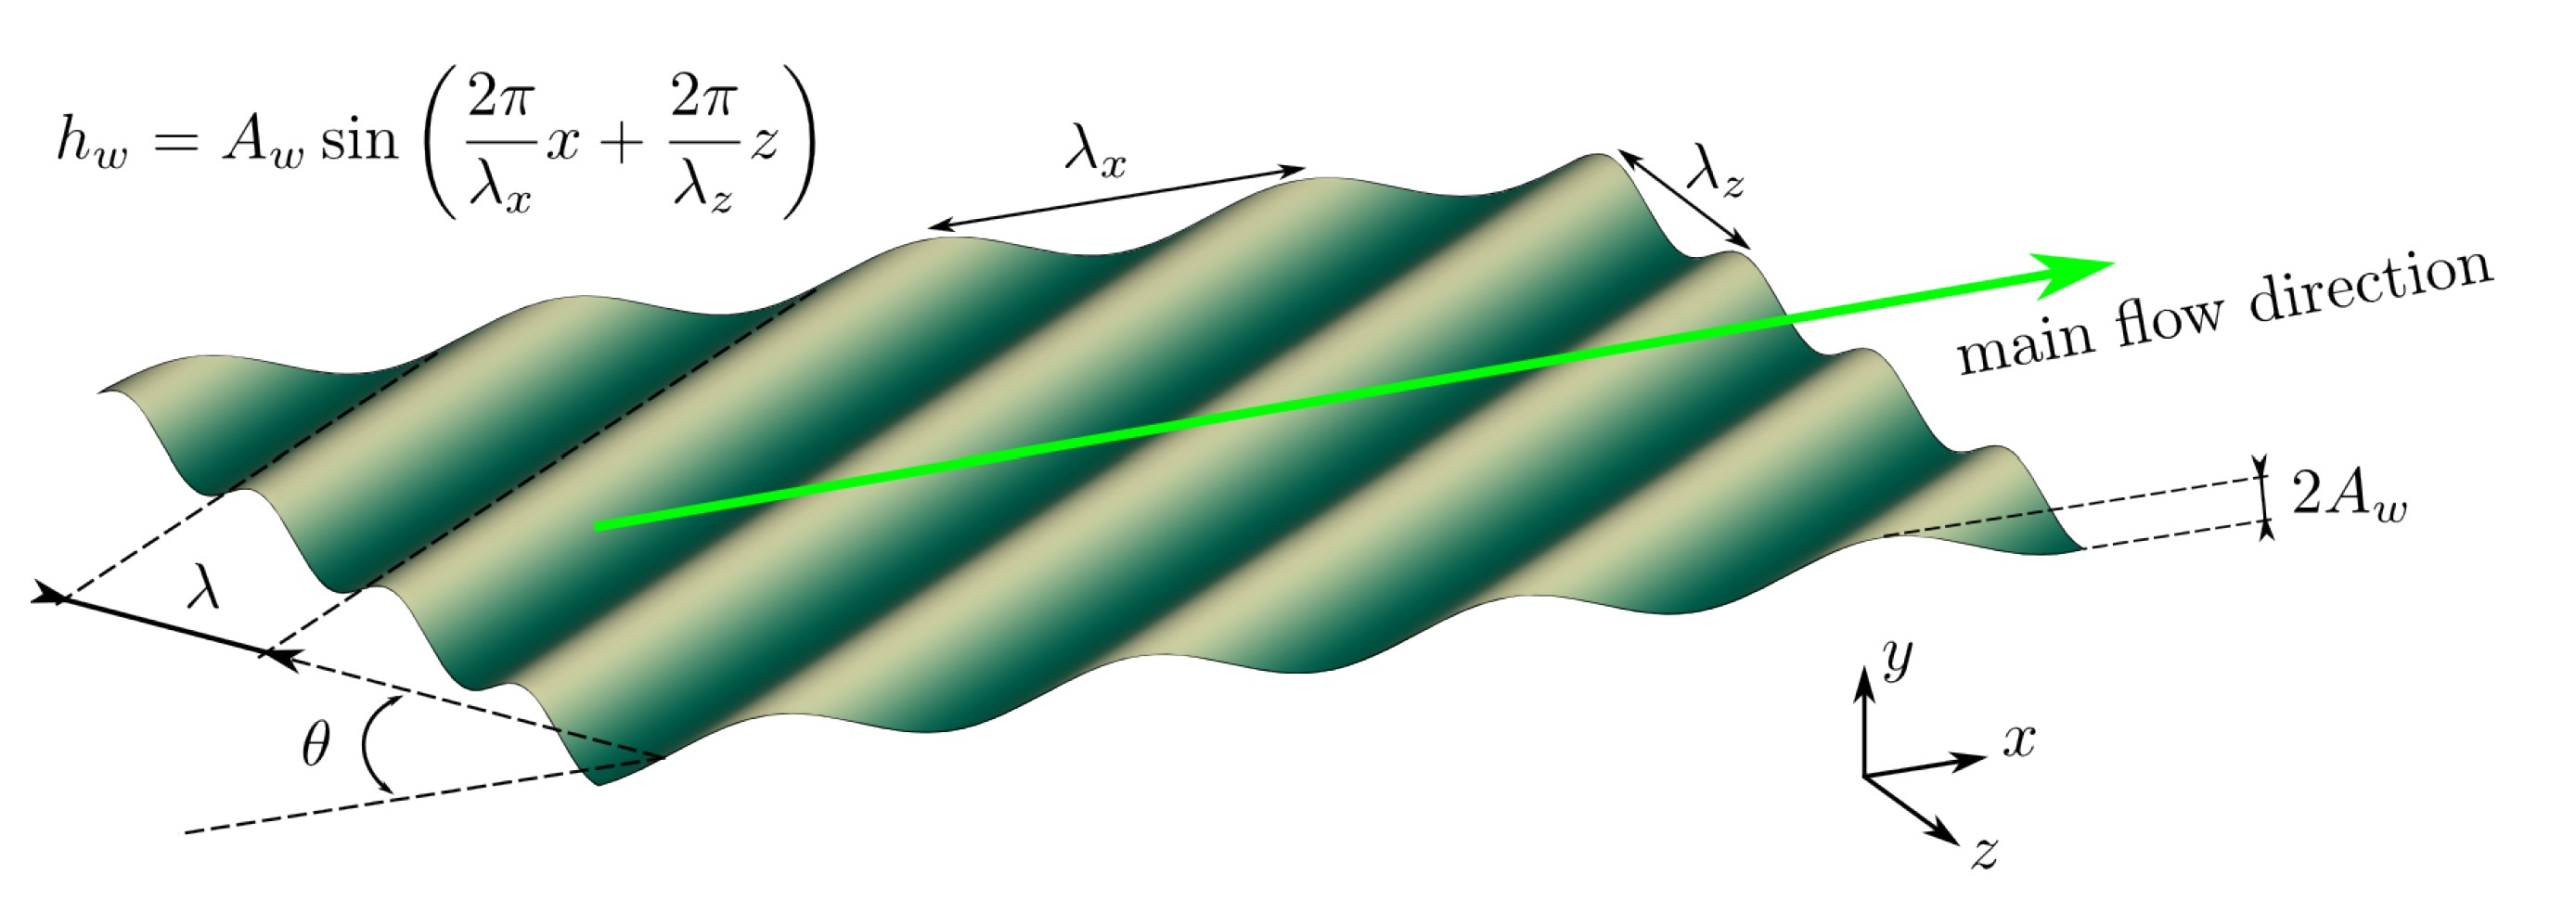
\includegraphics[width=0.7\linewidth]{introduction/fig/ww.jpg}
	\caption[Schematic of the oblique wavy wall]{Schematic of the oblique wavy wall from \cite{ghebali2018}. The green arrow represents the flow direction, at an oblique angle $\theta$ to the wavy wall.}
	\label{fig:ww}
\end{figure}
\begin{figure}[htbp]
	\centering
	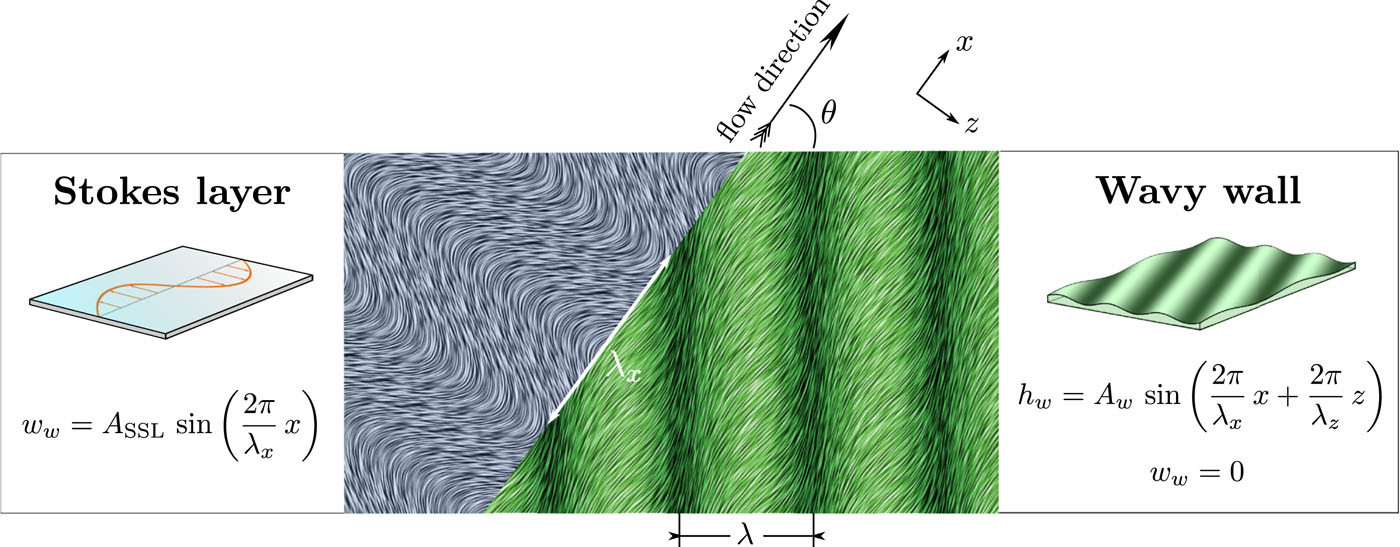
\includegraphics[width=0.9\linewidth]{introduction/fig/wwssl.jpeg}
	\caption[Comparison of mean streaklines close to the wall between SSL and WW]{An emulation of the forcing by \gls*{ssl} (left) and \gls*{ww} (right) showing mean streaklines close to the wall, where the background is coloured according to the norm of the velocity vector. Figure from \sgc. Here $A_w=\alpha$ from Figure~\ref{fig:ww}}
	\label{fig:sslwwcomparison}
\end{figure}

\subsubsection{Phase Averaged Velocity}
To find the net power reduction we again start with the \gls*{bl} equations linearised around a linear profile, Equations~\eqref{eq:blx}--\eqref{eq:blc}. However, since there are undulations along the wall, we will let the $y$ coordinate follow the contours of the wall. Hence by the no-slip and inpenetrability conditions, we have that at the wall $U\ww\pw=V\ww\pw=W\ww\pw=0$, and accordingly $\tilde{u}\ww\pw=\tilde{v}\ww\pw=\tilde{w}\ww\pw=0$ at the wall. Unlike the \gls*{ssl} case, we now have variations in pressure. This pressure variation is ``proportional to the velocity at the outer edge of the boundary layer and to the displacement magnitude'' and occurs as a result of the displacement of streamlines caused by variations in the shape of the wall surface, which ``is passed with little change to the streamlines at the outer edge of the boundary layer, where the flow velocity is large'' \cite{chernyshenko2013}. %(--------------------------------------------------------------------------------------------This can be shown with the bernoulli equation ----------------------------------------------------------------------)
This means that the phase averaged pressure does not vary in the wall normal direction and can then be assumed to have the form $\tilde{p}\pw\ww=\hat{P}\pw\ww e^{i\left( k_x\pw x\pw +k_z \pw z\pw \right) }$. The phase averaged velocity is a function of  $x,y,z$ and is then $\left( \tilde{u}\pw\ww,\tilde{w}\pw\ww,\tilde{w}\pw\ww \right) = \left( \hat{U}\ww\pw(y),\hat{V}\ww\pw(y),\hat{W}\ww\pw(y) \right)e^{i\left( k_x\pw x\pw +k_z \pw z\pw \right)} $. By substituting the above into the \gls*{bl} equations without the unnecessary  $y$-momentum equation, (i.e. Equations~\eqref{eq:blx},~\eqref{eq:blz},~\eqref{eq:blc}), we get
\begin{align}
	ik_x\pw y\pw \hat{U}\ww\pw+\hat{V}\ww\pw &= -ik_x\pw \hat{P}\ww\pw+\dv[2]{\hat{U}\ww\pw}{\left(y\pw\right)} \label{eq:blwwx}\\
	ik_x\pw y\pw \hat{W}\ww\pw &= -ik_z \hat{P}\ww\pw+\dv[2]{\hat{W}\pw\ww}{\left(y\pw\right)} \label{eq:blwwz}\\
	ik_x\pw \hat{U}\ww\pw + \dv{\hat{V}\ww\pw}{y\pw} + ik_z\pw \hat{W}\ww\pw &=0 \label{eq:blwwc}
.\end{align}
Now we eliminate $\hat{V}\ww\pw$ by substituting $\hat{V}\ww\pw$ from Equation~\eqref{eq:blwwx} into the second term of Equation~\eqref{eq:blwwc} to get
\begin{align}
	ik_x\pw \hat{U}\ww\pw + \dv{y\pw}(-ik_x\pw y\pw \hat{U}\pw\ww  -ik_x\pw \hat{P}\ww\pw+\dv[2]{\hat{U}\ww\pw}{\left(y\pw\right)}) + ik_z\pw \hat{W}\ww\pw &=0 \\
	ik_x\pw \hat{U}\ww\pw -ik_x\pw \left(\hat{U}\pw\ww+y\pw\dv{\hat{U}\pw\ww}{y\pw}\right)  +\dv[3]{\hat{U}\ww\pw}{\left(y\pw\right)} + ik_z\pw \hat{W}\ww\pw &=0 \\
	-ik_x\pw y\pw\dv{\hat{U}\pw\ww}{y\pw}  +\dv[3]{\hat{U}\ww\pw}{\left(y\pw\right)} + ik_z\pw \hat{W}\ww\pw &=0 \label{eq:blwwxc}
.\end{align}

We now let $y^{+}=\left( k_x^{+} \right) ^{-1 /3}y^{+}$ which we used in Section~\ref{sec:ssl} when we solved for the variation of spanwise velocity in $y$ for  \gls*{ssl} in order to make this calculation consistent with that of \gls*{ssl}. Furthermore, \textcite{chernyshenko2013} calculated that by rescaling as
\begin{equation}
	\hat{U}\pw\ww \left( y\pw \right)  = i\left( k_z\pw \right) ^2 \left( k_x\pw \right) ^{-5 /3}  \hat{P}\pw\ww \check{u}\pw\ww \left( \check{y}\pw \right)
,\end{equation}
and
\begin{equation}
	\hat{W}\pw\ww \left( y\pw \right) = ik_z\pw \left( k_x\pw \right) ^{-2 /3}\hat{P}\pw\ww \check{w}\pw\ww \left( \check{y}\pw \right)
,\end{equation}
we can substitute into Equation~\eqref{eq:blwwz} as
\begin{equation*}
	ik_x\pw \left[ \left( k_x\pw \right) ^{-1 /3} \check{y}\pw\right] \left[ i k_z\pw \left( k_x\pw \right) ^{-2 /3}\hat{P}\pw\ww \check{w}\pw\ww \right] = -ik_z \hat{P}\ww\pw\nonumber+\dv[2]{\left[i k_z\pw \left( k_x\pw \right) ^{-2 /3}\hat{P}\pw\ww \check{w}\pw\ww\right]}{\left(\left( k_x\pw \right) ^{-1 /3} \check{y}\pw\right)}
,\end{equation*}
and Equation~\eqref{eq:blwwxc} as
\begin{multline*}
	ik_x\pw \left[ \left( k_x\pw \right) ^{-1 /3} \check{y}\pw\right]\dv{\left[i\left( k_z\pw \right) ^2 \left( k_x\pw \right) ^{-5 /3}  \hat{P}\pw\ww \check{u}\pw\ww \right]}{\left( \left( k_x\pw \right) ^{-1 /3} \check{y}\pw\right)} - ik_z\pw \left[ ik_z\pw \left( k_x\pw \right) ^{-2 /3}\hat{P}\pw\ww \check{w}\pw\ww \right] \\
	=\dv[3]{\left[i\left( k_z\pw \right) ^2 \left( k_x\pw \right) ^{-5 /3}  \hat{P}\pw\ww \check{u}\pw\ww \right]}{\left( \left( k_x\pw \right) ^{-1 /3} \check{y}\pw\right)}
,\end{multline*}
to get
\begin{align}
	i\check{y}\pw \check{w}\pw\ww&=-1+\dv[2]{\check{w}\pw\ww}{\left( \check{y}\pw \right) }\label{eq:blwwzsim} \\
	\dv[3]{\check{u}\pw\ww}{\left( \check{y}\pw \right) } &= i\check{y}\pw \dv{\check{u}\pw\ww}{\check{y}\pw} -i\check{w}\pw\ww\label{eq:blwwxsim}
.\end{align}
This system has the boundary conditions $\dv{\check{u}\pw}{\check{y}\pw}\to0 $ and $\check{w}\to0$ as $\check{y}\pw\to\infty$, and $\check{u}\pw=\check{w}\pw=0$ and $\dv[2]{\check{u}\pw\ww}{\left( y\pw \right) } =\left(\frac{k_x\pw}{k_z\pw}\right)^2$ at $\check{y}\pw=0$. The final condition comes from solving Equation~\eqref{eq:blwwx} at $\check{y}\pw=0$ (where also $\hat{V}\pw\ww=0$).

Since Equation~\eqref{eq:blwwzsim} is decoupled from $\check{u}\pw\ww$, we can solve it numerically for $\check{w}\pw\ww$. Then to solve Equation~\eqref{eq:blwwx}, we decompose $\check{u}\pw\ww$ into
\begin{equation}
	\check{u}\pw\ww = \check{u}\pw_{w,\gls*{wv}}+\left( \frac{k_x\pw}{k_z\pw} \right) ^2\check{u}\pw_{p,\gls*{wv}}
,\end{equation}
with $\check{u}\pw_{w,\gls*{wv}}$ and $\check{u}\pw_{p,\gls*{wv}}$ satisfying
\begin{equation}
\dv[3]{\check{u}\pw_{w,\gls*{wv}}}{\left( \check{y}\pw \right) } =i\check{y}\pw \dv{\check{u}\pw_{w,\gls*{wv}}}{\check{y}\pw} -i\check{w}\pw\ww
,\end{equation}
where $\dv{\check{u}\pw_{w,\gls*{wv}}}{\check{y}\pw} \to 0\text{ as }\check{y}\pw\to\infty$, and $\check{u}\pw_{w,\gls*{wv}}=\dv[2]{\check{u}\pw_{w,\gls*{wv}}}{\left( \check{y}\pw \right) } =0$ at $\check{y}\pw=0$, and
\begin{equation}
	\dv[3]{\check{u}\pw_{p,\gls*{wv}}}{\left( \check{y}\pw \right) } =i\check{y}\pw \dv{\check{u}\pw_{p,\gls*{wv}}}{\check{y}\pw} 
,\end{equation}
where $\dv{\check{u}\pw_{p,\gls*{wv}}}{\check{y}\pw} \to 0\text{ as }\check{y}\pw\to\infty$, and $\check{u}\pw_{p,\gls*{wv}}=0$, $\dv[2]{\check{u}\pw_{p,\gls*{wv}}}{\left( \check{y}\pw \right) } =1 $ at $ \check{y}\pw=0$. Physically $\check{u}\pw_{w,\gls*{wv}}$ ``corresponds to the perturbation of $\left[u\ps\ww\right]$ due to wall-normal velocity induced by spanwise velocity dependence on  $z$'' whereas  $\check{u}\pw_{p,\gls*{wv}}$ ``is related to the perturbation of $\left[ u\ps\ww \right] $ due to the longitudinal pressure gradient induced by the wall'' \cite{chernyshenko2013}. These ordinary differential equations were then solved numerically by \textcite{chernyshenko2013} using Mathematica.

\subsubsection{Matching Spanwise Shear Profile with SSL}
In order to use the results of \textcite{viotti2009}, \textcite{chernyshenko2013} had the idea to matching the spanwise profiles between the \gls*{ssl} flow and the \gls*{ww} flow. In the ideal case, the spanwise velocities would be matched. However, at the wall, $\tilde{w}\ps\ssl\neq0$, whereas $\tilde{w}\pw\ww=0$ at the wall, which means we cannot possibly match the spanwise velocity profiles. So instead, they recognised that due to Galilean invariance, having similar motions in a different translated frame of reference will likely produce similar results. Therefore, instead the presumption was that having the same spanwise shear might affect turbulence the same way, leading to drag reduction. Thus, \textcite{chernyshenko2013} sought to match the \gls*{ssl} spanwise shear profile $\dv{\tilde{w}\ps\ssl}{y\ps} =\hat{W}\ps\ssl\dv{\check{w}\ps\ssl}{\check{y}\ps} e^{ik_x\ps x\ps}$ which is equivalent with
$\dv{\tilde{w}\pz\ssl}{y\pz} =\hat{W}\pz\ssl\dv{\check{w}\pz\ssl}{\check{y}\pz} e^{ik_x\pz x\pz}$
the \gls*{ww} spanwise shear profile $\dv{\tilde{w}\pw\ww}{y\ps}=ik_z\pw \left( k_x\pw \right) ^{-2 /3} \hat{P}\pw\ww \dv{\check{w}\pw\ww}{\check{y}\pw}  e^{i\left( k_x\pw x+k_z \pw z \right) }$. %(--------------------------------------)
Dependence on $z$ was neglected since $k_z\pw$ for the  \gls*{ww} is expected to be much larger than the characteristic scale of near wall turbulence. We know that streak spacing is around 100 wall units and their streamwise length is around 1000 wall units \cite{chernyshenko2005}; whereas the spanwise and streamwise wavelengths are expected to be on the same order, which from the \gls*{ssl} analysis in Section~\ref{sec:ssl} based on \textcite{viotti2009} is expected to be around 1000 wall units for optimal performance. On the contrary, a phase shift $\phi $ could be added between the \gls*{ssl} spanwise shear profile and that of the \gls*{ww}, as it would still produce the necessary profiles just further down the flow in the streamwise direction, since the thickness of the Stokes layer and the \gls*{ww} boundary layer are much smaller than the channel half-height \cite{ghebali2017}. Therefore, matching the spanwise shear profiles with a phase shift is equivalent to minimising the following equation
\begin{equation}
	\min \left\{ \int_{0}^{\infty} \int_{0}^{\frac{2\pi}{k_x^{+}}} \left| \dv{\check{w}\ps\ssl}{\check{y}\ps} e^{ik_x\ps x\ps} - \frac{ik_z\pw \left( k_x\pw \right) ^{-2 /3}\hat{P}\pw\ww }{\hat{W}\ps\ssl} \dv{\check{w}\pw\ww}{\check{y}\pw}  e^{i\left(k_x\pw x\pw+\phi \right)} \right|^2 \dd{x^{+}} \dd{y^{+}}  \right\}\label{eq:minshear}
\end{equation}
over $C=\frac{ik_z\pw \left( k_x\pw \right) ^{-2 /3}\hat{P}\pw\ww }{\hat{W}\ps\ssl}$ and $\phi $. Minimisation gave $C_\text{min} = 0.8980$ and $\phi _\text{min} =1.5708$, which is (interestingly) approximately $\frac{\pi}{2}$. Thus, to match the spanwise shear profiles, the amplitude of the periodic pressure field should be such that
\begin{equation}
	\hat{P}\pw\ww=C_\text{min} \frac{\hat{W}\ps\ssl}{ik_z\pw \left(k_x\pw\right)^{-2 /3}}\label{eq:phtselect}
.\end{equation}
Note that the \gls*{ww} height is unknown \text{a priori}, therefore it is likely that it would have to be picked by guessing, and trial and error via \gls*{dns}, \gls*{rans} simulations, or experiments to match the above periodic pressure field amplitude. The resulting spanwise shearprofile matching and its corresponding spanwise velocity are shown in Figures~\ref{fig:spanshearmatch} and~\ref{fig:spanvelmatch} respectively.

\begin{figure}[htbp]
	\centering
	\subfigure[Spanwise shear profiles.]{
		\label{fig:spanshearmatch}
		\def\svgwidth{.9\textwidth}
		\import{introduction/fig/spanshear/}{spanshearmatch.pdf_tex}
	}
	\subfigure[Spanwise velocity profiles.]{
		\label{fig:spanvelmatch}
		\def\svgwidth{.9\textwidth}
		\import{introduction/fig/spanvel/}{spanvelmatch.pdf_tex}
	}
	\caption[Spanwise shear and velocity profile comparison between SSL and WW]{Spanwise shear (a) and velocity (b) profile comparison between SSL (solid) and WW (dashed) using $\Re \left\{ \check{w}\ps\ssl (\check{y}\ps)e ^{ik_x\ps x\ps} \right\} $ and $\Re \left\{ C_\text{min} \check{w}\pw\ww (\check{y}\pw)e ^{ik_x\pw x\pw} \right\} $ respectively for velocity, and their derivatives with respect to $\check{y}^{+}$ for shear at $\frac{k_x^{+}x^{+}}{2\pi}=0, \frac{1}{6}, \frac{2}{6}, \frac{3}{6}, \frac{4}{6},$ and $\frac{5}{6}$ from left to right.}
	\label{fig:spanmatch}
\end{figure}

\subsubsection{Net Power Reduction for WW}
Similar to the  \gls*{ssl} flow discussed in Section~\ref{sec:ssl}, we will define the net power reduction as a percentage of the power required to drive the reference channel flow as
\begin{align}
	P_\text{net,\gls*{wv}} &\equiv P_\text{sav,\gls*{wv}} +P_\text{req,\gls*{wv}} \\
			       &\equiv 100\% \frac{\Delta \Phi _{\overline{U},\gls*{wv}}\pz+\Delta \Phi_{\mathbf{u'} ,\gls*{wv}}\pz }{\Phi \zz\pz} +100\% \frac{\Delta \Phi _{\tilde{\mathbf{u} },\gls*{wv}}\pz}{\Phi \zz\pz}
,\end{align}
where $\Delta \Phi _{\overline{U},\gls*{wv}}\pz=\Phi _{\overline{U},\gls*{zer}}\pz-\Phi _{\overline{U},\gls*{wv}}\pz $, $\Delta \Phi_{\mathbf{u'} ,\gls*{wv}}\pz =\Phi_{\mathbf{u'} ,\gls*{zer}}\pz -\Phi_{\mathbf{u'} ,\gls*{wv}}\pz $, and unlike \gls*{ssl}, with two phase averaged components $\Delta \Phi _{\tilde{\mathbf{u} },\gls*{wv}}=-\left(\Phi _{\tilde{u},\gls*{wv}}+\Phi _{\tilde{w},\gls*{wv}}\right)$. Unlike \gls*{ssl}, $P_\text{req} $ is no longer the power required for the actuator to create the spanwise forcing, but is instead the extra power required by the hypothetical pump driving the main flow to overcome the phase averaged forcing in both the streamwise direction and the spanwise direction, the latter of which we have previously attempted to match to \gls*{ssl} as closely as possible.

Armed with the definition, it is known that at high Reynolds numbers, the differences in $\overline{U}^{+}$ is negligible. Therefore, in \textcite{chernyshenko2013}, without even mentioning it specifically, it was assumed that the difference in mean velocity profiles between the reference and controlled flows were the same, i.e. $\Delta \Phi _{\overline{U},\gls*{wv}}=\Delta \Phi _{\overline{U},\gls*{sl}}$. Moreover, because of the matching of spanwise shear, it is therefore assumed that the effects on the stochastic turbulence leading to drag reduction is the same and therefore that $\Delta \Phi _{\mathbf{u'} ,\gls*{wv}}=\Delta \Phi _{\mathbf{u'} ,\gls*{sl}}$. Therefore, \textcite{chernyshenko2013} claimed that
\begin{equation}
	P_\text{sav,\gls*{wv}} = P_\text{sav,\gls*{sl}}  
.\end{equation}

However, we do expect some change in the net power usage due to the presence of changing pressure gradients. The difference in power reduction, therefore, comes in the $P_\text{req,\gls*{wv}} $ term. According to \sct, for a \gls*{ww} the dissipation due to phase averaged velocity gradients are given by %(----------------------------------------------------------sdakf ---------------------------------------------------------------safkl idk-------------------------------------)

%Thus,
%\begin{align}
%	\Phi _{\tilde{u},\gls*{wv}}\pw &= \int_{0}^{\infty} \overline{\left( \dv{\tilde{u}\ww\pw}{y\pw}  \right) ^2} \dd{y\pw}   \\
%				       &= \int_{0}^{\infty} \left( \dv{\overline{i\left( k_z\pw \right) ^2 \left( k_x\pw \right) ^{-5 /3}  \hat{P}\pw\ww \check{u}\pw\ww e^{i\left( k_x\pw x\pw +k_z \pw z\pw \right)}}}{\left((k_x\pw)^{-1 /3}\check{y}\pw\right)}  \right) ^2 \dd{\left(\left(k_x\pw\right)^{-1 /3}\check{y}\pw\right)}   \\
%				       &= \left(k_z\pw\right)^4\left(k_x\pw\right)^{-3}\hat{P}\ww\pw\int_{0}^{\infty}\frac{1}{2} \left| \dv{\check{u}\ww\pw}{\check{y}\pw}  \right| ^2 \dd{\check{y}\pw} \label{eq:fiwwpwu}
%.\end{align}
%\begin{align}
%	\Phi _{\tilde{w},\gls*{wv}}\pw &= \int_{0}^{\infty} \overline{\left( \dv{\tilde{w}\ww\pw}{y\pw}  \right) ^2} \dd{y\pw}   \\
%				       &= \int_{0}^{\infty} \left( \dv{\overline{ik_z\pw \left( k_x\pw \right) ^{-2 /3}\hat{P}\pw\ww \check{w}\pw\ww e^{i\left( k_x\pw x\pw +k_z \pw z\pw \right)}}}{\left((k_x\pw)^{-1 /3}\check{y}\pw\right)}  \right) ^2 \dd{\left(\left(k_x\pw\right)^{-1 /3}\check{y}\pw\right)}   \\
%				       &= \left(k_z\pw\right)^{2}\left(k_x\pw\right)\hat{P}\ww\pw\int_{0}^{\infty}\frac{1}{2} \left| \dv{\check{w}\ww\pw}{\check{y}\pw}  \right| ^2 \dd{\check{y}\pw} \label{eq:fiwwpww}
%.\end{align}
\begin{align}
	\Phi _{\tilde{u},\gls*{wv}}\pw&=k_z\pw \left(k_x\pw\right)^{-2 /3} \hat{P}\ww\pw \int_{0}^{\infty} \frac{1}{2} \left| \dv{\check{u}\ww\pw}{\check{y}\pw}  \right| d\check{y}\pw,\\
	\Phi _{\tilde{w},\gls*{wv}}\pw&=k_z\pw \left(k_x\pw\right)^{-2 /3} \hat{P}\ww\pw \int_{0}^{\infty} \frac{1}{2} \left| \dv{\check{w}\ww\pw}{\check{y}\pw}  \right| d\check{y}\pw,\\
.\end{align}

By selecting  $\hat{P}\ww\pw$ using Equation~\eqref{eq:phtselect}, we are guaranteeing that $\Phi _{\tilde{w},\gls*{wv}}\pw\leq\Phi _{\tilde{w},\gls*{sl}}\ps$. This is because by optimising over $C$ in Equation~\eqref{eq:minshear} ``is equivalent to projecting the \gls*{ssl} solution onto the direction of the wavy-wall solution in the $L_2$ functional space'' \cite{chernyshenko2013}, i.e. it is equivalent to projecting the \gls*{ssl} spanwise shear profile as a vector in the direction of that of \gls*{ww}, which is necessarily equal or less than the magnitude of the \gls*{ssl} vector. To be safe in their calculations, \textcite{chernyshenko2013} therefore assumed the maximum value of $\Phi _{\tilde{w},\gls*{sl}\ps}\pz$ which is equal to $\Phi _{\tilde{w},\gls*{sl}}\pz$. Thus,
\begin{equation}
	P_\text{req,\gls*{wv}} = 100\% \frac{-\left(\Phi _{\tilde{u},\gls*{wv}}\pz+\Phi _{\tilde{w},\gls*{wv}}\pz\right)}{\Phi \zz\pz}
	= -100\% \frac{\Phi _{\tilde{u},\gls*{wv}}\pz+\Phi _{\tilde{w},\gls*{wv}}\pz}{\Phi _{\tilde{w},\gls*{wv}}\pz}\frac{\Phi _{\tilde{w},\gls*{sl}}\pz}{\Phi \zz\pz}
	= \frac{\Phi _{\tilde{u},\gls*{wv}}\pw+\Phi _{\tilde{w},\gls*{wv}}\pw}{\Phi _{\tilde{w},\gls*{wv}}\pw}P_\text{req,\gls*{sl}}
.\end{equation}

Defining the squared norm $\|\cdot\|^2\equiv \int_{0}^{\infty} \left( \cdot \right) ^{2} \dd{y}  $, we can define a ratio $r$ as follows
\begin{equation}
	r\equiv\frac{\Phi _{\tilde{u},\gls*{wv}}\pw+\Phi _{\tilde{w},\gls*{wv}}\pw}{\Phi _{\tilde{w},\gls*{wv}}\pw}=\frac{\|\hat{W}\pw\ww\|^2+\|\hat{U}\pw\ww\|^2}{\|\hat{W}\pw\ww\|^2}=1+\left( \frac{k_x\pw}{k_z\pw} \right) ^{-2} \frac{\|\check{u}_{w,\gls*{wv}}\pw+\left( \frac{k_x\pw}{k_z\pw} \right) ^2 \check{u}_{p,\gls*{wv}}\pw\|^2}{\|\check{w}\ww\pw\|^2}
.\end{equation}
Since they are fractions, the non-dimensionalisation by wall units here is unnecessary but included for clarity. $r$, as it turns out, is only dependent on $\frac{k_x\pw}{k_z\pw}$; numerically determining the norms, it was found that
\begin{equation}
	r=3.122+2.323 \left( \frac{k_x\pw}{k_z\pw} \right) ^2+0.7986 \left( \frac{k_x\pw}{k_z\pw} \right) ^{-2} 
.\end{equation}
By minimising $r$, we minimise $P_\text{req,\gls*{wv}} $. This is given by
\begin{equation}
	r_\text{min} =5.846 \text{ at } \frac{k_x\pw}{k_z\pw}\rvert_\text{opt} = 0.7657 \implies \theta_\text{opt} = \ang{52.56}
,\end{equation}
where $\theta_\text{opt} $ is the optimal oblique angle of the \gls*{ww} to the streamwise direction.

Finally, with $P_\text{net,\gls*{wv}} = P_\text{sav,\gls*{wv}} +P_\text{req,\gls*{wv}} =P_\text{sav,\gls*{sl}} +rP_\text{req,\gls*{sl}} $, and the known results of the latter three terms from this section and Section~\ref{sec:ssl}, we can estimate the net power reduction of th \gls*{ww} flow as compared to the reference flow. This is plotted in Figure~\ref{fig:pnet} for the prescribe $\hat{W}\pz\ssl=2,6$ for $ P_\text{sav,\gls*{wv}}=P_\text{sav,\gls*{sl}} $. It was shown that $\hat{W}\pz\ssl=2$ gives the best result at $\lambda_x\pz=1520$ of a net power savings due to drag reduction of 2.4\% compared to the reference flow. Moreover, \gls*{dns} of the flow at $\Rey_{\tau}\approx180$ at approximately these optimal conditions gave $r=5.4$ \cite{ghebali2018}, which is similar to that we found as $r_\text{min} $.


\subsection{CFD Results of the Wavy Wall (WW)}\label{sec:cfdww}
\textcite{ghebali2017} performed \gls*{dns} of the \gls*{ww} at $ \gls*{ret}\approx360$, which is incredibly computationally expensive as it requires a large domain, especially since the domain now has to accommodate for the spanwise wavelength of the \gls*{ww}, which is an order of magnitude larger than the spanwise spacing of streaks \cite{chernyshenko2005}. This means that only a few configurations were tested, and that so-far this is the only detailed numerical simulation of the \gls*{ww}. The change in $ \gls*{ret}$ as compared to that of \vqt, which used $ \gls*{ret}=200$, is assumed to not have significant impact on the optimal wavelength \sgc. Strangely, they found that as mesh size of the domain is refined, the predicted drag reduction decreases. The maximum net drag reduction was found to be 0.7\% with a 2\% friction drag reduction and 1.3\% pressure drag penalty, at a configuration of wall height amplitude $\alpha\pw\approx 20,$ \gls*{ww} angle  $\theta=\ang{70}$, and \gls*{ww} streamwise wavelength $\lambda\pw_x\approx920$ \sgc. Although it ``appears to tend, asymptotically to a positive value of 0.6\%'' under the configuration of \sgc. Higher friction drag reduction by increasing height amplitude is possible, but comes at a great cost of pressure drag. \textcite{vannesselrooij2016} showed that dimpled surfaces for drag reduction cannot be too high as separation occurs, what's more is that the adverse pressure gradient becomes stronger, which generates instabilities via different mechanisms therefore changing the total drag reduction. %(---------------------------no citation-----------------------------------------------)
This value of 0.6\% was therefore thought to be the maximum possible net drag reduction, which is significantly lower than the 2.4\% predicted by \textcite{chernyshenko2013} with a different $\theta$.

This discrepancy is believed to have potentially come from the assumption that $P_\text{sav,\gls*{wv}}= P _\text{sav,\gls*{sl}} $. \textcite{gatti2016} examined the effects of Reynolds number on turbulent skin-friction drag reduction using spanwise forcing. They found that at low Reynolds numbers, $\gls*{ret}\approx200$, which is the regime for which these analyses were conducted, the vertical shift of the logarithmic portion of the mean streamwise velocity profile did not stay constant. Therefore, it is believed that the assumption that $\overline{U}\pw\ww=\overline{U}\ps\ssl$ is in fact untrue, and therefore the resulting change in dissipation due to the mean profile is also false.

\section{Problem Formulation}\label{sec:objective}\glsreset{dr} \glsreset{ww}
The main objective of this project is to be able to predict an estimate of the net \gls*{dr} due to the \gls*{ww} for a given wavy wall prescribed by $k_x\pz$, $k_z\pz$, and the corresponding $\hat{W}\pz\ssl$ at $ \gls*{ret}=200$ using only the curve fitted to $P_\text{sav,\gls*{sl}} $ \gls*{dns} data from \vqt. A first attempt at this objective was already done by \sct, and relayed again in Section~\ref{sec:ww} of this report. However, as outlined in Section~\ref{sec:cfdww}, we believe there was an error in the assumptions made; in that at these low Reynolds numbers the changes in dissipation due to mean streamwise velocity profile between two similar flows cannot be ignored. This report will therefore show our attempts to take the changes into account.

%To do so (------------------------------ sections 1, 2, 3----------------)

%Intro: Motivation, Riblets, and others in general, Lit Review – Stokes Layer Results; SSL+Chernyshenko. Refer to Ghebali DNS. End:Formulation of problem: want to be able to predict drag reduction by WW as f’n of $k_x, k_z$, and What



%It is known that if in a turbulent flow the (wing) surface moves spanwise with a suitable velocity distribution, the friction drag is significantly reduced. Even though causing the wing surface to move requires energy input, the drag reduction is large enough to provide large energy savings. However, such motion is difficult to implement on an aircraft. In a paper (Chernyshenko, 2013, arxiv.org/abs/1304.4638) it was proposed to shape the rigid (not moving) surface in such a way that the resulting fluid motion will emulate the effect of the surface motion without the surface actually moving. For the case of the surface with sinusoidal waves at an angle to the mean flow direction, an optimisation of the angle and the height of the waves was performed. The later comparisons (Ghebali et al., 2017, aip.scitation.org/doi/10.1063/1.5003617) showed that the semi-empirical model of calculating the drag reduction used for optimisation was inaccurate. This might be due to this model not taking into account the energy dissipation due to the laminar viscosity and the shape of the mean velocity profile. This part of the dissipation is negligible at high Reynolds numbers, but it was significant at the Reynolds numbers studied. The project will consist in improving the semi-empirical model and repeating the shape optimisation using the improved model. It is recommended to see the first paper cited above to estimate the degree of mathematical proficiency needed for this project.


%This is one of the most important components of the dissertation. It should begin with a clear statement of what the project is about so that the nature and scope of the project can be understood by a lay reader. It should summarise everything you set out to achieve, provide a clear summary of the project's background and relevance to other work and give pointers to the remaining sections of the dissertation which contain the bulk of the technical material.
%
%Further information can be found here: \url{https://goo.gl/k2huN9}.
%
%\section{\LaTeX{} code examples and formatting tips}
%Hello, here's a citation \cite{greenwade93}. References are stored in a Bibtex file. Google Scholar and IEEExplore allow you to download citations of papers in Bibtex format from their search engine. Some people use JabRef (\url{http://www.jabref.org}) to manage their database of references.
%
%This is an inline equation $\Gamma(t)=K_i e^{\sin^2(\omega_t)}$. The first paragraph appears without indent but the following ones will have an indentation.
%
%This is an actual named equation:
%\begin{equation}
%v(x)=\frac{1}{2}\sin(2 \omega t + \phi) e^{-j s t}
%\label{eq:cacona}
%\end{equation}
%\noindent where $\omega$ is the angular speed. Notice that symbols liks $\omega$ should be written in italics whereas measurement units such as V for Volts appear as normal text. This paragraph didn't have an indentation because the first sentence was linked to the definition of equation (\ref{eq:cacona}). A code snippet for an example program is shown in Listing~\ref{lst:code1}.
%
%\begin{lstlisting}[caption=Source code for {\it hello.m},label=lst:code1,breaklines=true,basewidth=4pt,prebreak=**,postbreak=**,frame=single]
%for i:=maxint to 0 do
%begin
%{ do nothing }
%end;
%Write('Case insensitive ');
%Write('Pascal keywords.');
%\end{lstlisting}
%
%The characteristic parameters of the system are sumarised in Table~\ref{tab:tab1}. A figure is shown Fig~\ref{fig:felix}, we don't necessarily know if this figure will appear below, above or elsewhere; therefore, the text should never refer to the figure with sentences such as {\it "As shown here:"}.
%%
%\begin{figure}[htbp]
%\centering
%
\includegraphics[width=0.3\linewidth]{introduction/fig/Felix_the_cat.pdf}
%\caption{Felix the Cat}
%\label{fig:felix}
%\end{figure}
%
%\begin{table}[htbp]
%	\centering
%	\begin{tabular}{lll}
%		Parameter & Value & Units\\
%		\hline
%		$P$ & 1 & kW \\
%		$Q$ & 0 & kVAr\\
%	    \hline
%	\end{tabular}
%	\caption{Characteristic parameters of the system}
%	\label{tab:tab1}
%\end{table}
%
%\begin{samepage}
%Sometimes, the symbols in an equation are defined as follows\footnote{Some authors like to define their symbols this way.}:
%\begin{equation}
%	V(t)=A \sin(\omega t+\theta_0)
%\end{equation}
%\begin{tabular}{lll}
%	where & $V$ & is a voltage waveform,\\
%	& $A$ & is the amplitude of the voltage,\\
%	& $\omega$ & is the angular frequency,\\
%	& $t$ & is the time.
%\end{tabular}
%\end{samepage}
%
%\subsection{A brief comparison between a proper plot and a horrible plot}
%
%Figure~\ref{fig:fig2} contains two plots of the same waveform. Subfigure~\ref{fig:fig2sub1} shows a badly formatted figure, Subfigure~\ref{fig:fig2sub2} shows a much better formatted figure. The problems with Subfigure~\ref{fig:fig2sub1}, listed by order or relevance, are the following:
%
%\begin{enumerate}
%    \item The font size is too small to be read properly.
%    \item The axes aren't labeled properly: the horizontal axis is not labeled and the units of the vertical axis are unknown. Further, symbols must be written in italics whereas numbers and units must be written as normal text.
%    \item The choice of limits for the axes is not good, the figure has wide useless empty spaces. The most relevant part of the waveform is the transient that happens between times $t=$0 and $t=$0.05 s, which is less than 10\% of the timespan shown in the figure.
%    \item The figure has been scaled without keeping the original aspect ratio and fonts look narrower than they would if the figure had been scaled properly.
%    \item The plot doesn't have grid lines. This makes it hard to read the exact value (ie time, voltage) of points in the trace.
%    \item The width of the trace is too thin and may not be visible if printed in low resolution.
%    \item The choice of units of the vertical axis aren't the best. For example, in this case the plot would be easier to read if voltage had been expressed in kV instead of V.
%    \item The figure was exported as a bitmap (e.g. png, jpg, bmp) instead of being exported in vector format (e.g. eps, svg, pdf) and visual artifacts appear when the figure is scaled up or down in order to fit in the document.
%\end{enumerate}
%
%\begin{figure}[htbp]
%	\centering
%	\subfigure[A horrible one.]{
%		\label{fig:fig2sub1}
%        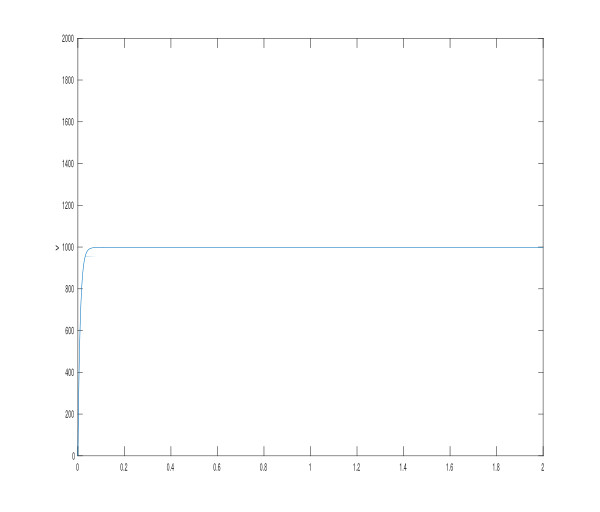
\includegraphics[width=0.5\linewidth]{introduction/fig/figure1.jpg}}
%	\subfigure[A proper one.]{
%		\label{fig:fig2sub2}
%		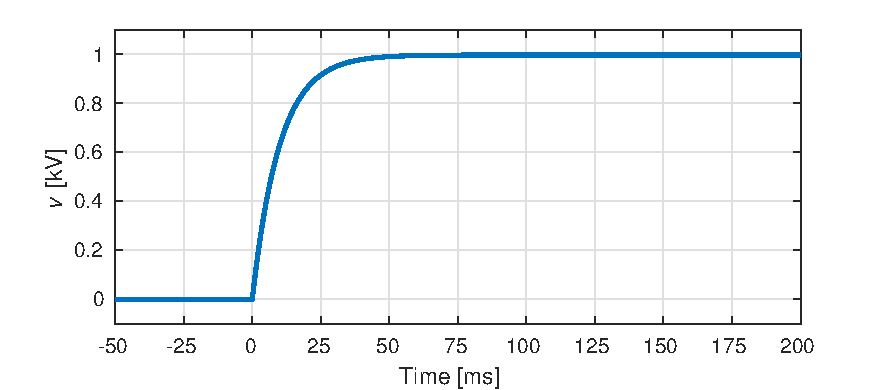
\includegraphics[width=0.6\linewidth]{introduction/fig/figure2.pdf}}
%	\caption{A figure with two subfigures.}
%	\label{fig:fig2}
%\end{figure}
%
%\begin{landscape}
%	\begin{figure}[htbp]
%\centering
%
\includegraphics[width=0.5\linewidth]{introduction/fig/Felix_the_cat.pdf}
%\caption{Here's a large drawing of Felix the Cat that wouldn't fit in a portrait page}
%\label{fig:felix2}
%\end{figure}
%\end{landscape}
%
%\section{Objectives}
%\section{Challenges}
%\section{Contributions}
